\documentclass[aspectratio=169]{beamer}

\usepackage{amsmath,amssymb}
\usepackage{booktabs}
\usepackage{tabularx}
\usepackage[table,svgnames]{xcolor}
\usepackage{tikz}
\usetikzlibrary{arrows.meta,backgrounds,calc,positioning,shapes.multipart,fit}
\usepackage[shorthands=off,main=spanish]{babel}
\usepackage{ragged2e}

\definecolor{fortranPurple}{HTML}{503874}
\definecolor{fortranPurpleMid}{HTML}{7E5AA6}
\definecolor{rakaliOrange}{HTML}{D9542B}

\usetheme[
  accent=fortranPurple,
  progressbar=foot,
  sectionpage=progressbar,
  numbering=fraction,
  numberrail=section,
  block=fill,
  notes=hide,
  closing=contact
]{cookie}

% Preamble (once):
%   \usepackage[table,svgnames]{xcolor}
%   \usepackage{booktabs}
%   \usepackage{tabularx}
\definecolor{cDone}{HTML}{8FD9A8}
\definecolor{cWip} {HTML}{F4C95D}
\definecolor{cTodo}{HTML}{E8918C}
\newcommand{\yes}[1]{\cellcolor{cDone}#1}
\newcommand{\prt}[1]{\cellcolor{cWip}#1}
\newcommand{\nope}[1]{\cellcolor{cTodo}#1}



\title[Fortran]{¿Quién necesita C++? }
\subtitle{Fortran al rescate para programar CPUs y GPUs de manera portable}
\author[Jorge Luis Gálvez Vallejo \textperiodcentered\ NCI]{Jorge Luis Gálvez Vallejo \textnormal{(NCI)}}
\cookieemail{jorge.galvezvallejo@anu.edu.au}
\institute{NCI}
\cookieuni{Australian National University}
\cookielocation{Canberra, Australia}
\date{\today}
\cookietagline{}

\titlegraphic{%
  \begin{tabular}{@{}c@{}}
    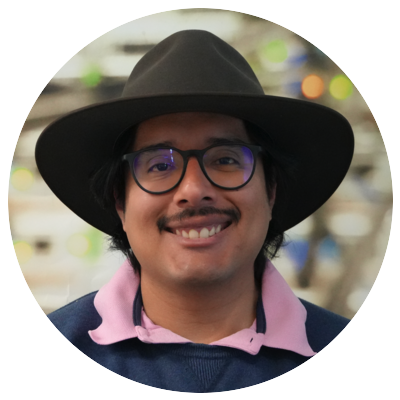
\includegraphics[height=1.6cm]{assets/jorge_c.png}\\[.7em]
    
\includegraphics[height=1.0cm]{assets/nci.png}
  \end{tabular}%
}

\cookieclosingtitle{Gracias}
\cookieclosingtext{No todo necesita Fortran, pero no tampoco todo necesita C++.}
\cookieclosingqr{https://github.com/JorgeG94/pic}
\cookieclosingqrlabel{github.com/JorgeG94/pic}

\begin{document}

\maketitle

% =====================================================================
\section{Casi 70 años}

\begin{frame}{El lenguaje de alto nivel más viejo del mundo}
  \centering
  \begin{tikzpicture}
    \draw[cookie arrow,line width=1pt] (-0.7,0) -- (11.7,0);
    \foreach \x/\y/\t in {%
      0/1957/{Fortran},%
      2.75/1990/{arrays de\\primera clase},%
      5.5/2003/{orientación\\a objetos},%
      8.25/2008/{\texttt{do concurrent}\\coarrays},%
      11/{2018--2023}/{interop.\ con C\\mejoras a DC}} {
      \fill[fortranPurple] (\x,0) circle (2.6pt);
      \node[font=\small\bfseries,above=2.5mm,text=fortranPurple] at (\x,0) {\y};
      \node[font=\scriptsize,below=2.5mm,align=center,text width=2.5cm] at (\x,0) {\t};
    }
  \end{tikzpicture}
  \vspace{1.4em}
  \begin{exampleblock}{}
    \centering No es un lenguaje viejo. Es un lenguaje \textbf{con historia}. \\
    {\footnotesize Casi todo lo que la gente critica de Fortran se decidió \textbf{antes de 1990}.}
  \end{exampleblock}
\end{frame}

\begin{frame}{La mala fama}
  \vspace{.5em}
  \begin{columns}[T,onlytextwidth]
    \column{.49\textwidth}
      \begin{alertblock}{Problemas de verdad}
        \begin{itemize}\setlength\itemsep{2pt}
          \item \textbf{Compiladores}: una pesadilla: GNU, Intel, NVIDIA, Cray, AMD, Flang
          \item \textbf{Compatibilidad}: el código de 1980 todavía compila --- y el lenguaje carga con todo
        \end{itemize}
      \end{alertblock}
    \column{.49\textwidth}
      \begin{alertblock}{Y el problema de fondo}
        \begin{itemize}\setlength\itemsep{2pt}
          \item Cada vez \textbf{menos usuarios}
          \item \textbf{La docencia se fue}: métodos numéricos y física computacional
            ahora se enseñan con Python, C++, Julia
        \end{itemize}
      \end{alertblock}
  \end{columns}
  \vspace{.4em}
  {\footnotesize\itshape C y C++ se volvieron la alternativa para el cálculo científico moderno.
  Fortran perdió la clientela.}
\end{frame}

\begin{frame}{Sin embargo}
  \begin{columns}[T,onlytextwidth]
    \column{.48\textwidth}
      \begin{itemize}\setlength\itemsep{3pt}
        \item Arrays de primera clase --- rebanadas, \texttt{elemental}, reducciones, sin escribir el loop 
        \item Orientación a objetos \cookiebadge{F2003}
      \end{itemize}
    \column{.48\textwidth}
      \begin{itemize}\setlength\itemsep{3pt}
        \item Memoria dinámica (casi) segura --- \texttt{allocatable}, \texttt{move\_alloc}
        \item Paralelismo nativo \textbf{en el estándar} \cookiebadge{F2008}
      \end{itemize}
  \end{columns}
  \vfill
  \begin{exampleblock}{El meollo del asunto:}
    \centering Fortran permite escribir código eficiente sin tener que haber estudiado ciencias de la computación.
  \end{exampleblock}
\end{frame}

% =====================================================================
\section{Un solo código}

\begin{frame}[fragile]{El mismo loop donde sea!}
  \begin{columns}[T,onlytextwidth]
    \column{.52\textwidth}
      \begin{cookiecode}[title=Fortran estándar]{Fortran}
do concurrent (k=1:nk,j=1:nj,i=1:ni)
  c(i,j,k) = al*a(i,j,k) + b(i,j,k)
end do
      \end{cookiecode}
    \column{.46\textwidth}
      \begin{cookiecode}[title=El muro de directivas]{Fortran}
!$omp target teams loop collapse(3)
do k = 1, nk
  do j = 1, nj
    do i = 1, ni
      c(i,j,k) = alpha*a(i,j,k) + b(i,j,k)
    end do
  end do
end do
      \end{cookiecode}
  \end{columns}
  \vspace{.3em}
  
\end{frame}

\begin{frame}{Dónde sí y dónde no?}{Cada vendor hace offload a \emph{su} GPU }
  \centering
  \scalebox{0.86}{\input{compiler_table_body.tex}}
\end{frame}

\begin{frame}{Coarrays}
  \begin{columns}[T,onlytextwidth]
    \column{.5\textwidth}
      \begin{block}{La promesa}
        {\footnotesize F2008. El diseño es \textbf{elegante}: memoria distribuida
        dentro del lenguaje, sin biblioteca externa.}
      \end{block}
    \column{.48\textwidth}
      \begin{alertblock}{La realidad}
        {\footnotesize GCC necesita OpenCoarrays. Intel trae el suyo. El de Cray es bueno.
        \textbf{NVIDIA y AMD prácticamente no existen}.}
      \end{alertblock}
  \end{columns}
  \vspace{.5em}
  \begin{exampleblock}{Mi modelo mental no es: ``nativo es bueno''}
    \centering Es: \textbf{portable y listo para la vida real, o no cuenta}. \\
    {\footnotesize \texttt{do concurrent} lo pasa. Los coarrays \emph{todavía} no.}
  \end{exampleblock}
  \vspace{.3em}
  {\footnotesize Para memoria distribuida uso \textbf{MPI}; por eso existe \texttt{pic-mpi}.
  Podría añadirle un backend de coarrays --- decidí que no: la mayoría de los runtimes de
  coarrays están implementados \textbf{sobre MPI}, así que estaría envolviendo una envoltura.}
\end{frame}

% =====================================================================
\section{Rakali}

\begin{frame}{Rakali: una historia de éxito}{Simulación hidrodinámica --- costas, ríos, inundaciones, océano abierto --- 100\% Fortran}
  \begin{columns}[T,onlytextwidth]
    \column{.55\textwidth}
      \centering
      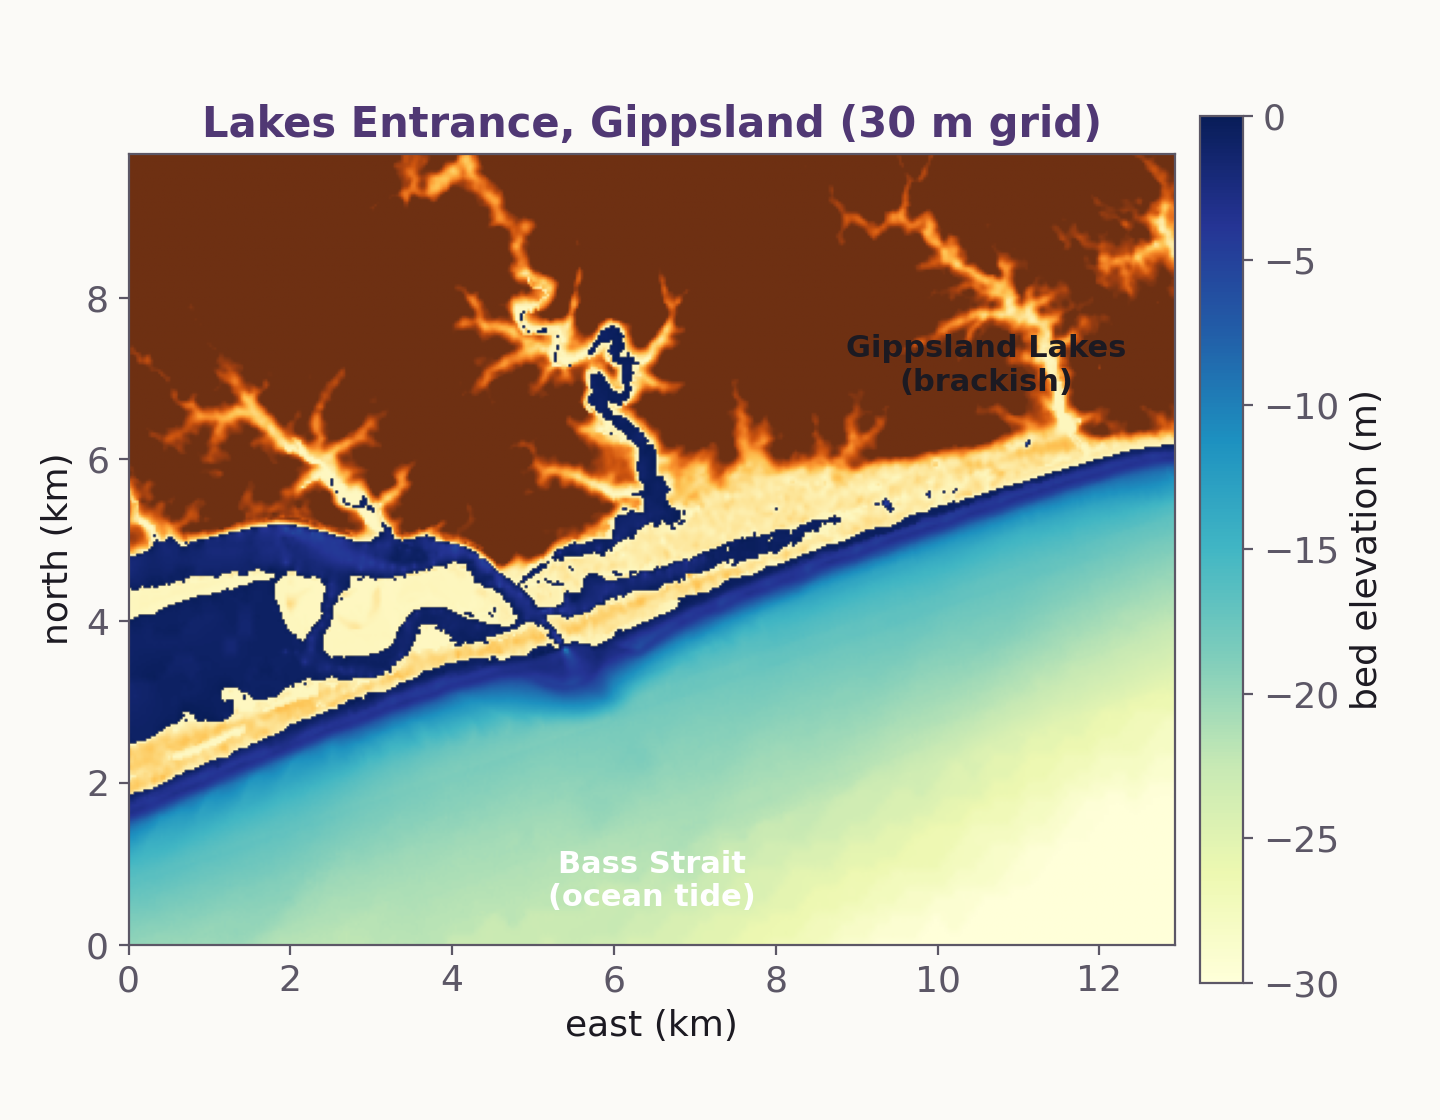
\includegraphics[width=\textwidth,height=.66\textheight,keepaspectratio]{assets/fig_setting.png}
    \column{.43\textwidth}
      \begin{itemize}\setlength\itemsep{3pt}
        \item Lakes Entrance, Gippsland
        \item Malla de \textbf{30\,m}
        \item Marea del estrecho de Bass contra los lagos salobres
      \end{itemize}
      \vspace{.4em}
      \begin{block}{Portabilidad real}
        {\footnotesize
        \textbf{GPUs}: NVIDIA, AMD, Intel \\[.2em]
        \textbf{CPUs}: Apple, ARM, Intel, AMD \\[.35em]
        Un solo código fuente.}
      \end{block}
  \end{columns}
\end{frame}

\begin{frame}{Los números}
  \begin{columns}[T,onlytextwidth]
    \column{.5\textwidth}
      \centering
      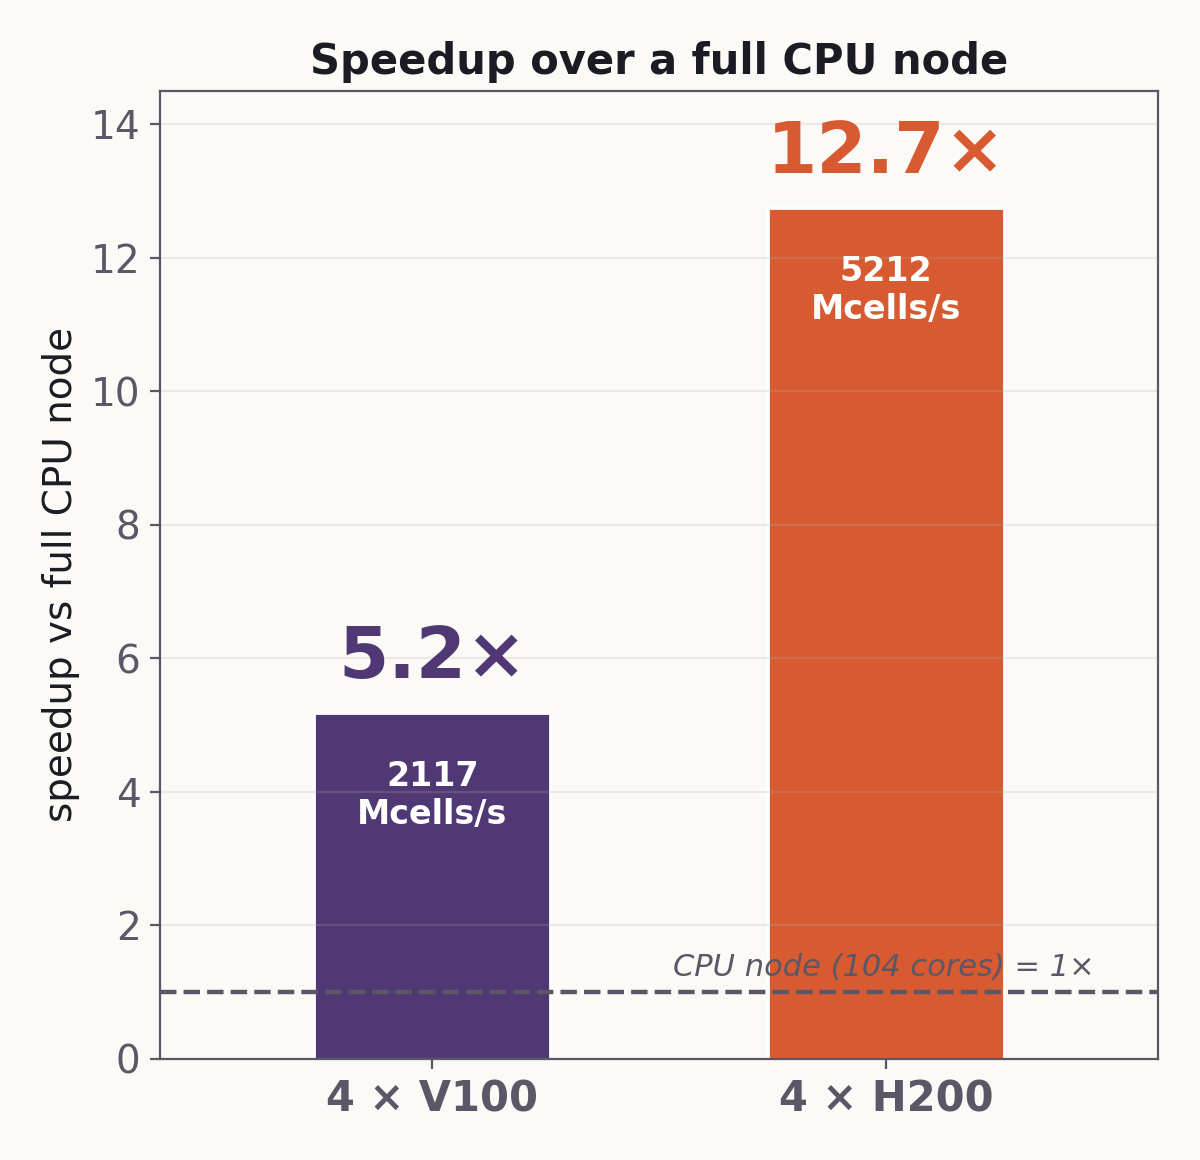
\includegraphics[width=\textwidth,height=.68\textheight,keepaspectratio]{assets/fig_speedup.png}
    \column{.48\textwidth}
      \centering
      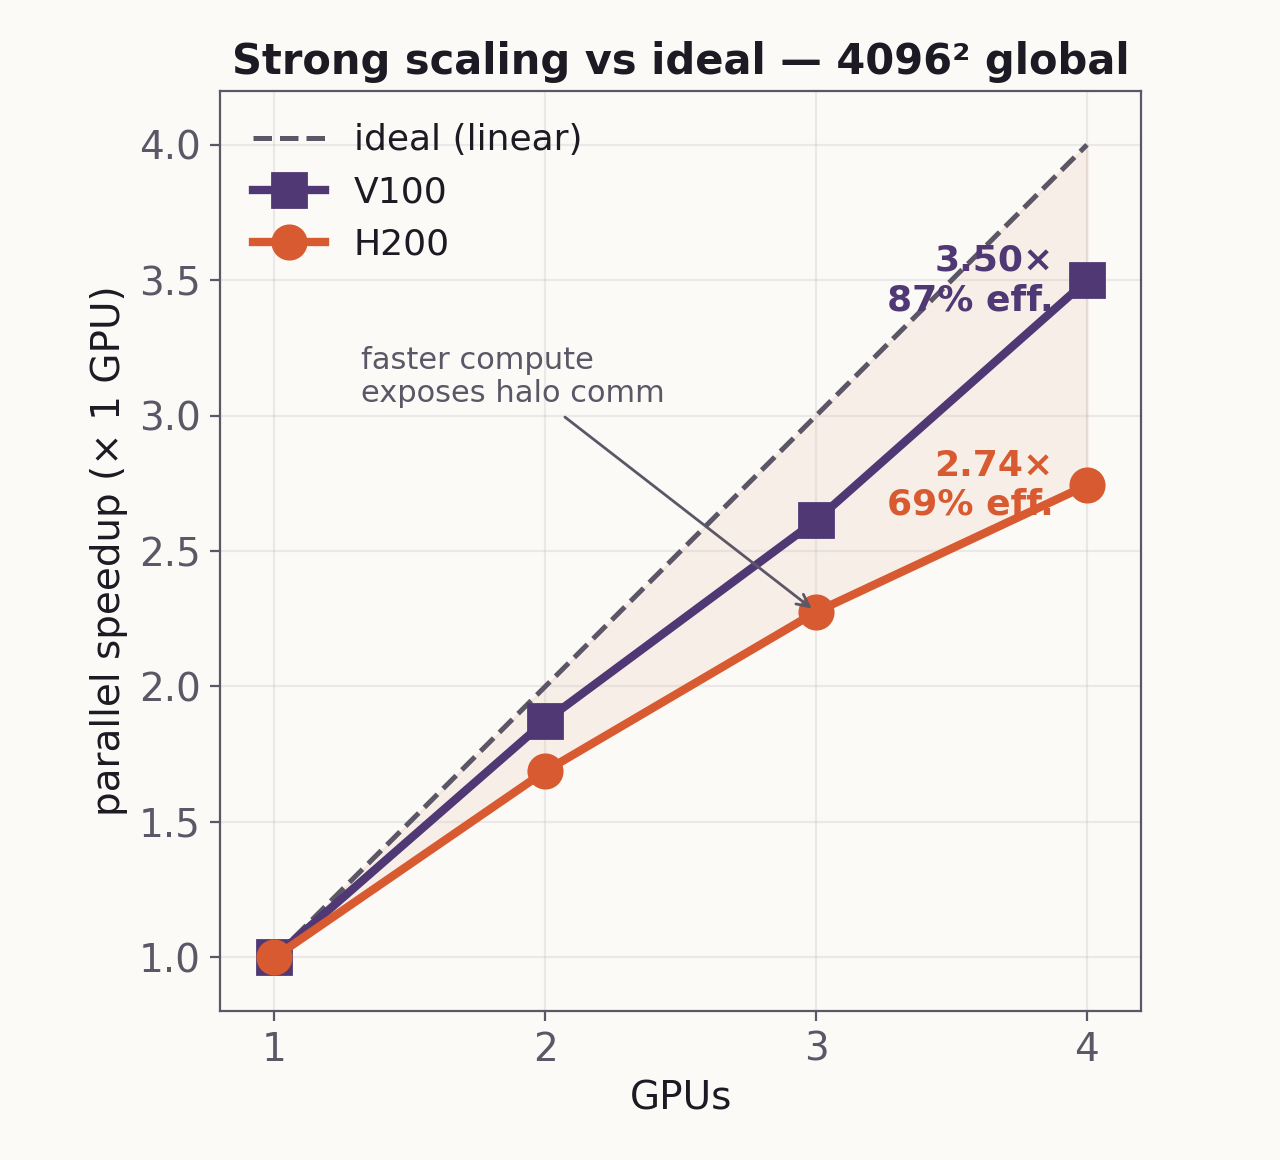
\includegraphics[width=\textwidth,height=.68\textheight,keepaspectratio]{assets/fig_strong_scaling.png}
  \end{columns}
  \vspace{.2em}
  {\footnotesize Contra un nodo CPU completo (104 núcleos): \textbf{5.2$\times$} con 4$\times$V100,
  \textbf{12.7$\times$} con 4$\times$H200.}
\end{frame}

\begin{frame}{La parte honesta}
  \begin{columns}[T,onlytextwidth]
    \column{.52\textwidth}
      \begin{alertblock}{Mejor hardware, peor eficiencia}
        {\footnotesize
        Escalamiento fuerte a 4 GPUs: \\[.3em]
        V100 --- \textbf{87\%} de eficiencia \\
        H200 --- \textbf{69\%} de eficiencia \\[.4em]
        El cómputo más rápido \textbf{expone la comunicación de halos}.}
      \end{alertblock}
    \column{.46\textwidth}
      \begin{block}{Por qué lo cuento}
        {\footnotesize Ante un público de ingeniería de software, el resultado que \emph{no}
        salió como uno quería vale más que el que sí.}
      \end{block}
  \end{columns}
  \vfill
\end{frame}

% =====================================================================
\section{Lo que costó}

\begin{frame}{El lenguaje es portable. El ecosistema no.}
  Rakali funciona. Pero \textbf{mantenerlo} reveló el problema de fondo:
  \vspace{.5em}
  \begin{itemize}\setlength\itemsep{4pt}
    \item \textbf{stdlib} es muy buena --- y en la práctica compila con GNU
    \item \texttt{mpi\_f08} necesita \textbf{vapaa} (Hammond) para cruzar compiladores
    \item Cada proyecto reimplementa las mismas cinco cosas: ordenamiento, logging,
      timers, strings, pegamento para BLAS
  \end{itemize}
  \vfill
  \begin{exampleblock}{}
    \centering Ese hueco es de \textbf{ingeniería}, no de ciencia. \\
    {\footnotesize Y por eso es nuestro trabajo.}
  \end{exampleblock}
\end{frame}

\begin{frame}{El ecosistema pic}
  \centering
  \begin{tikzpicture}[node distance=5mm]
    \node[cookie accent node,align=center,minimum width=9.2cm,minimum height=1.05cm] (pic)
      {\textbf{pic} --- rutinas nivel stdlib en Fortran nativo \\ \footnotesize ordenamiento \textperiodcentered\ arrays \textperiodcentered\ strings \textperiodcentered\ loggers \textperiodcentered\ timers};
    \node[cookie node,align=center,minimum width=2.9cm,minimum height=.95cm,above left=6mm and 0mm of pic.north west,anchor=south west] (blas) {\textbf{pic-blas}\\\footnotesize BLAS portable};
    \node[cookie node,align=center,minimum width=2.9cm,minimum height=.95cm,right=3mm of blas] (mpi) {\textbf{pic-mpi}\\\footnotesize distribuido};
    \node[cookie node,align=center,minimum width=2.9cm,minimum height=.95cm,right=3mm of mpi] (dev) {\textbf{pic-device}\\\footnotesize capa de dispositivo};
    \node[align=center,minimum width=9.2cm,minimum height=.8cm,below=6mm of pic,font=\footnotesize,draw=cookieMuted,rounded corners=3pt] (interop)
      {interoperabilidad, porque nunca estás atrapado: \textbf{libfint} (libcint, portado) \textperiodcentered\ interfaz a \textbf{cuEST}};
    \draw[cookie arrow] (blas.south) -- (blas.south |- pic.north);
    \draw[cookie arrow] (mpi.south)  -- (mpi.south  |- pic.north);
    \draw[cookie arrow] (dev.south)  -- (dev.south  |- pic.north);
  \end{tikzpicture}
  \vspace{.6em}

  \cookiebadge{fpm} \hspace{.3em}\cookiebadge{CMake} \hspace{.3em}\cookiebadge{compilar en todos lados!}
\end{frame}

\begin{frame}{No es una biblioteca de conveniencia: es infraestructura}
  \begin{columns}[T,onlytextwidth]
    \column{.48\textwidth}
      \begin{block}{metalquicha}
        {\footnotesize Química cuántica. Tres motores (\texttt{tblite}, \texttt{libcint},
        \texttt{cuEST}) tras \textbf{una sola interfaz}. \\[.3em]
        El camino CPU existe para \textbf{estar en desacuerdo} con el de GPU ---
        y todo se valida contra PySCF.}
      \end{block}
    \column{.48\textwidth}
      \begin{block}{terco}
        {\footnotesize Integrales de repulsión electrónica en GPU, \textbf{solo con
        \texttt{do concurrent}}. \\[.3em]
        Una \textbf{V100 de 2017}: \textbf{3.5$\times$} más rápido que Q-Chem con
        104 hilos en Sapphire Rapids.}
      \end{block}
  \end{columns}
  \vfill
  \begin{exampleblock}{}
    \centering Hidrodinámica y química cuántica sobre la misma base. \\
    {\footnotesize Eso es lo que convierte a \texttt{pic} en infraestructura.}
  \end{exampleblock}
\end{frame}

\begin{frame}{Cierre}
  \begin{cookiequote}
    Si ignoramos la propaganda contra Fortran , hay un lenguaje muy poderoso al alcance de cualquiera.
  \end{cookiequote}
  \vspace{.6em}
  \centering
  Pero no se sostiene solo. Necesita \textbf{CI}, \textbf{empaquetado}, \textbf{pruebas}, \textbf{diseño de APIs}.

  \vspace{.8em}
  {\large C++ no tiene todas las respuestas. Tiene más \textbf{ingeniería}.}

  \vspace{1em}
  {\footnotesize
  \texttt{pic} \textperiodcentered\ \texttt{pic-blas} \textperiodcentered\ \texttt{pic-mpi} \textperiodcentered\ \texttt{pic-device} \\
  \texttt{rakali} \textperiodcentered\ \texttt{metalquicha} \textperiodcentered\ \texttt{terco} \textperiodcentered\ \texttt{libfint} \\[.4em]
  \texttt{github.com/JorgeG94} \textperiodcentered\ \texttt{fortran-lang.org}}
\end{frame}

\appendix

\begin{frame}{Respaldo: MOM6, un tercer testigo}
  \begin{itemize}
    \item \textbf{200 mil líneas} de código climático que \emph{no} escribí
    \item Mismo enfoque: \texttt{do concurrent} para el cómputo, directivas solo para mover datos
    \item Requisito heredado y no negociable: \textbf{reproducibilidad bit a bit}
  \end{itemize}
  \vfill
  {\footnotesize\itshape Clima y química cuántica, códigos distintos, misma conclusión.}
\end{frame}

\end{document}
